%\chapter{3D-Stereokalibrierung und Szenenrekonstruktion mit reellen Daten und Kameras unterschiedlicher Auflösung}
\label{sec:realAuf} 

\section{Ergebnisse einer Stereoanalyse mit Kameras unterschiedlicher Auflösung}

Für den Test, ob Szenerekonstruktion im Realbeispiel auch mit unterschiedlichen Kameraauflösungen funktioniert, wurde eine der von Matlab ermittelten Kameramatrizen $K'$ und auch die durch den Surf Algorithmus detektierten Punkte jeweils skaliert. mn Kapitel \nameref{sec:basisTransformation} wurden die einzelnen Bauteile der Kameramatrix genau beschrieben. Die Kameramatrix $K'$ aus Matlab für die Canon 60D gegeben.


\begin{gather}
		K'=\begin{bmatrix}
\alpha_x&s&x_{0}\\
0&\alpha_y&y_{0}\\
0&0&1
\end{bmatrix}
\end{gather} \\

$\alpha_x$ und $\alpha_y$ setzen sich auch dem Abstand des Kamerazentrums zum Hauptpunkt zusammen, welcher in dieser Arbeit als mit $\zeta$ bezeichnet wurde, und den Kantenlängen der Pixel auf dem Sensor $m_x$ und $m_y$. Um die Auflösung der Kamera zu verändern, wird auf $\alpha_x$ und $\alpha_y$ jeweils ein beliebiger Faktor dazu multipliziert. Zum Beweis, dass die Rekonstruktion der externen Kameraparameter und die Szenerekonstruktion, bei egal welcher Skalierung, die ähnlichen Ergebnisse liefern, wurde die Kameramatrix $K'$ mit den Verhältnissen $[2:2], \, [5:2],\, [2:1], \, [1:2]$ und $[1.2:2.3]$ skaliert. 

\begin{gather*}
K'_{[2:2]}=	
\begin{bmatrix}
\alpha_x \cdot 2 &s&x_{0} \cdot 2\\
0&\alpha_y \cdot 2&y_{0} \cdot 2\\
0&0&1
\end{bmatrix}\\
K'_{[5:2]}=	
\begin{bmatrix}
\alpha_x \cdot 5 &s&x_{0} \cdot 5\\
0&\alpha_y \cdot 2&y_{0} \cdot 2\\
0&0&1
\end{bmatrix}\\
K'_{[2:1]}=	
\begin{bmatrix}
\alpha_x \cdot 2 &s&x_{0} \cdot 2\\
0&\alpha_y \cdot 1&y_{0} \cdot 1\\
0&0&1
\end{bmatrix}\\
K'_{[1:2]}=	
\begin{bmatrix}
\alpha_x \cdot 1 &s&x_{0} \cdot 1\\
0&\alpha_y \cdot 2&y_{0} \cdot 2\\
0&0&1
\end{bmatrix}\\
K'_{[1.2:2.3]}=	
\begin{bmatrix}
\alpha_x \cdot 1.2 &s&x_{0} \cdot 1.2\\
0&\alpha_y \cdot 2.3&y_{0} \cdot 2.3\\
0&0&1
\end{bmatrix}\\
\end{gather*}

Die Formulierung, dass die jeweils neu rekonstruierten Szenen ähnlich sind, wurde deshalb verwendet, da durch die zuvorigen Fehler der korrespondierenden Punkte und später, bei der Triangulierung, durch die \textit{Sampson-Approximation} Abweichungen auftreten können. Als Beweise werden im folgenden vier Beispiele für die vier Lösungen der rekonstruierten Translationsmatrizen $R'$ aufgezeigt. Des Weiteren werden die 3D-Plots und 2D-Plots der rekonstruierten Szenen bei unterschiedlich Auflösungen im Vergleich mit der Szene bei gleichen Auflösungen gezeigt. Die Koordinaten sind in unskalierten Pixeleinheiten gegeben. Die Originalszene ist in Abbildung 7.15 und 7.16 zu sehen. Zu beachten ist, das die Ausgabe des 3D Plots in \textit{Mathematica} manchmal rechtsdrehend, manchmal linksdrehend dargestellt sind, weshalb der Eindruck aufkommt, die Szene und die Kameraposition seien gespiegelt dargestellt. Dies leider auf ein generellen Darstellungsproblem von 3D-Plots in Mathematica zurückzuführen. Dieses kann mit zusätzlichem Code bereinigt werden, wurde aber zu diesem Zeitpunkt noch nicht implementiert. 


\begin{figure}[!htb]
	\minipage{0.48\textwidth}
	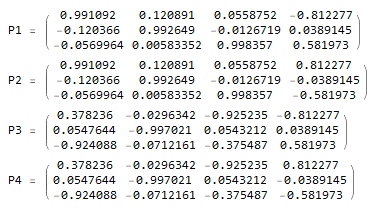
\includegraphics[width=\linewidth]{images/R_11.png}
	\caption{Zeigt die Die rekonstruierte Matrix $R'$ bei unveränderter Auflösung. Die Auflösungen von $C_\delta$ und $C'_\delta$ sind die selben.}
	\label{fig:awesome_image1}
	\endminipage\hfill
	\minipage{0.48\textwidth}
	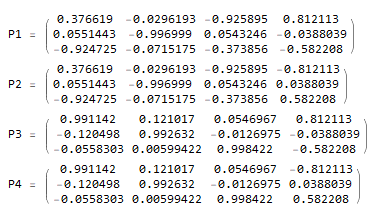
\includegraphics[width=\linewidth]{images/R_52.png}
	\caption{Zeigt die rekonstruierte Matrix $R'$ wenn $K'$ mit einem Verhältnis von $[5:2]$ skaliert wurde}
	\label{fig:awesome_image2}
	\endminipage\hfill
\end{figure}

\begin{figure}[!htb]
	\minipage{0.48\textwidth}
	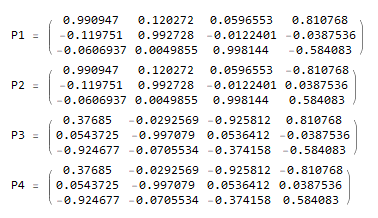
\includegraphics[width=\linewidth]{images/R_12.png}
	\caption{Zeigt die rekonstruierte Matrix $R'$ wenn $K'$ mit einem Verhältnis von $[1:2]$ skaliert wurde}
	\label{fig:awesome_image1}
	\endminipage\hfill
	\minipage{0.48\textwidth}
	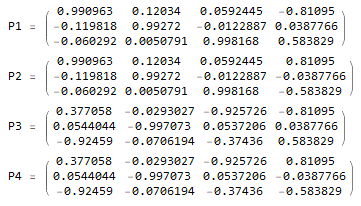
\includegraphics[width=\linewidth]{images/R_12_23.png}
	\caption{Zeigt die rekonstruierte Matrix $R'$ wenn $K'$ mit einem Verhältnis von $[1.2:2.3]$ skaliert wurde}
	\label{fig:awesome_image2}
	\endminipage\hfill
\end{figure}


\begin{figure}[!htb]
	\minipage{0.48\textwidth}
	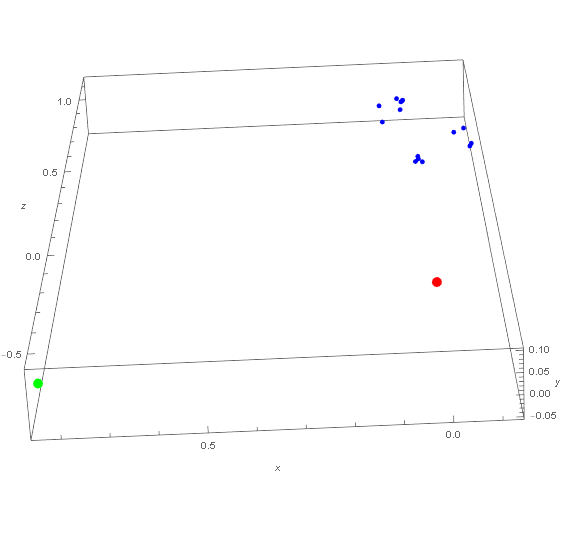
\includegraphics[width=\linewidth]{images/Reconstrution3D_52.png}
%	\caption{$C$ und $C'$ haben die selbe Auflösung eingestellt}
	\label{fig:awesome_image1}
	\endminipage\hfill
	\minipage{0.48\textwidth}
	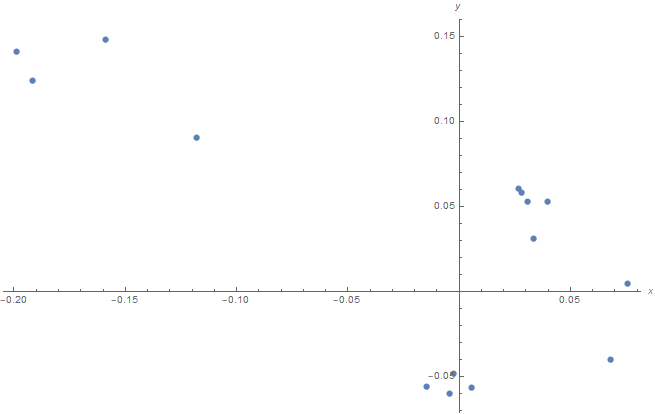
\includegraphics[width=\linewidth]{images/Reconstrution2D_52.png}
%	\caption{$C$ und $C'$ haben unterschiedliche Auflösungen eingestellt}
	\label{fig:awesome_image2}
	\endminipage\hfill
	\caption{Rekonstruierte Szene, wenn $K'$ mit einem Verhältnis von $[5:2]$ skaliert wurde}
\end{figure}
\begin{figure}[!htb]
	\minipage{0.48\textwidth}
	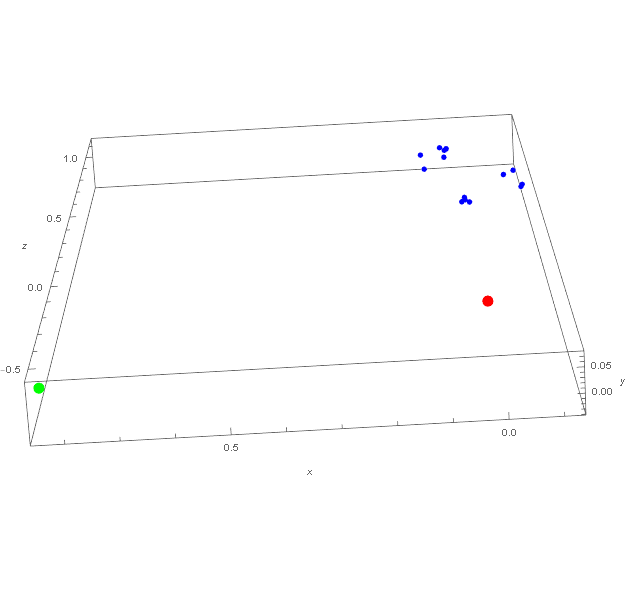
\includegraphics[width=\linewidth]{images/Reconstrution3D_21.png}
	%	\caption{$C$ und $C'$ haben die selbe Auflösung eingestellt}
	\label{fig:awesome_image1}
	\endminipage\hfill
	\minipage{0.48\textwidth}
	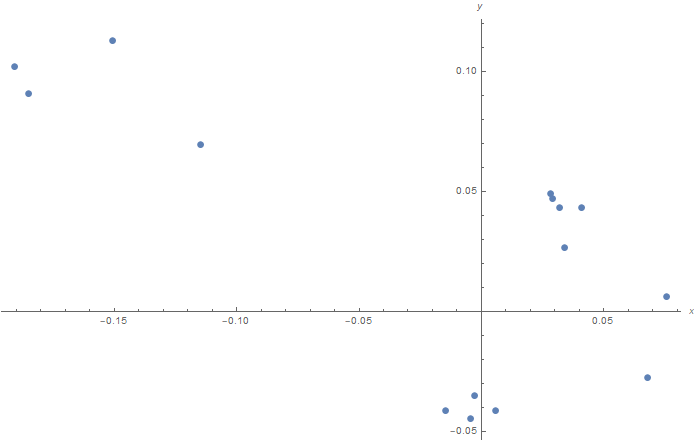
\includegraphics[width=\linewidth]{images/Reconstrution2D_21.png}
	%	\caption{$C$ und $C'$ haben unterschiedliche Auflösungen eingestellt}
	\label{fig:awesome_image2}
	\endminipage\hfill
	\caption{Rekonstruierte Szene, wenn $K'$ mit einem Verhältnis von $[2:1]$ skaliert wurde}
\end{figure}
\begin{figure}[!htb]
	\minipage{0.48\textwidth}
	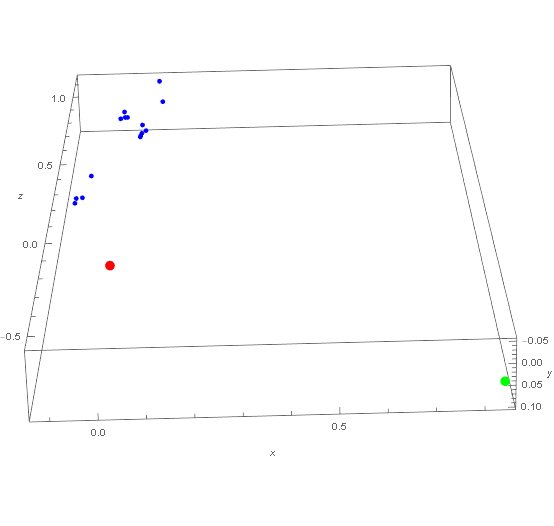
\includegraphics[width=\linewidth]{images/Reconstrution3D_12.png}
	%	\caption{$C$ und $C'$ haben die selbe Auflösung eingestellt}
	\label{fig:awesome_image1}
	\endminipage\hfill
	\minipage{0.48\textwidth}
	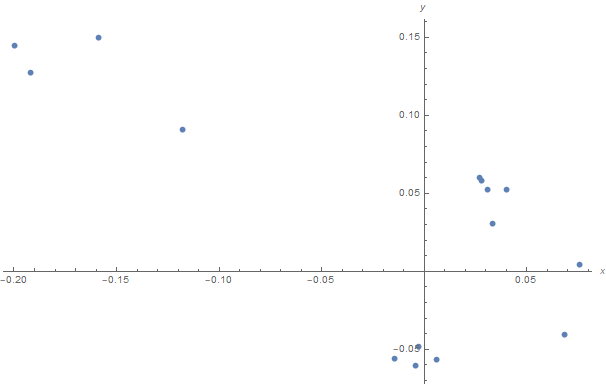
\includegraphics[width=\linewidth]{images/Reconstrution2D_12.png}
	%	\caption{$C$ und $C'$ haben unterschiedliche Auflösungen eingestellt}
	\label{fig:awesome_image2}
	\endminipage\hfill
	\caption{Rekonstruierte Szene, wenn $K'$ mit einem Verhältnis von $[1:2]$ skaliert wurde}
\end{figure}
\begin{figure}[!htb]
	\minipage{0.48\textwidth}
	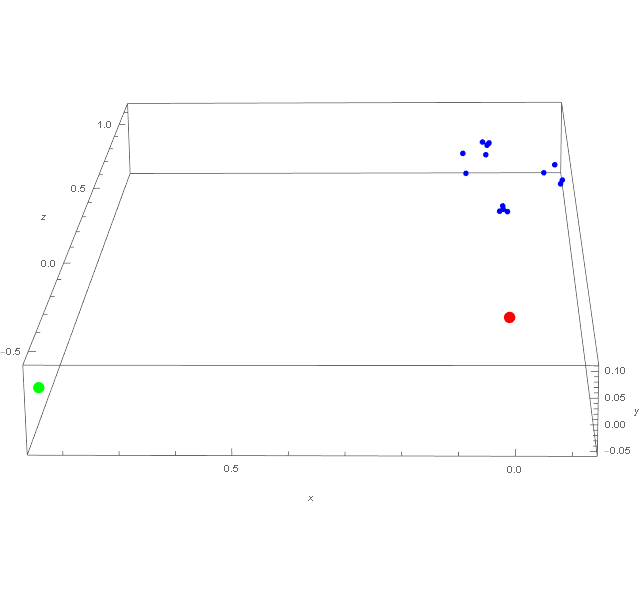
\includegraphics[width=\linewidth]{images/Reconstrution3D_12_23.png}
	%	\caption{$C$ und $C'$ haben die selbe Auflösung eingestellt}
	\label{fig:awesome_image1}
	\endminipage\hfill
	\minipage{0.48\textwidth}
	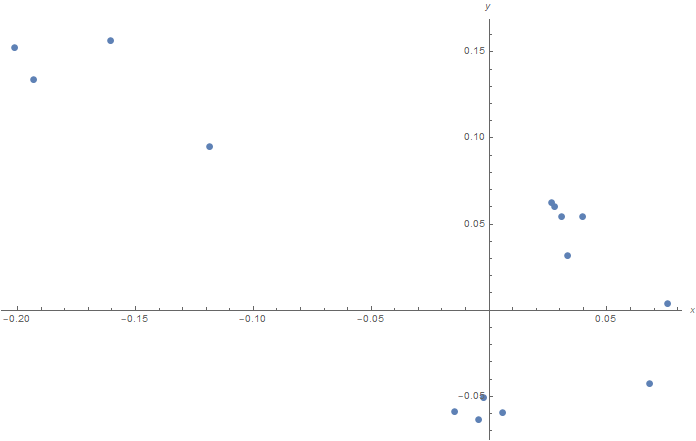
\includegraphics[width=\linewidth]{images/Reconstrution2D_12_23.png}
	%	\caption{$C$ und $C'$ haben unterschiedliche Auflösungen eingestellt}
	\label{fig:awesome_image2}
	\endminipage\hfill
	\caption{Rekonstruierte Szene, wenn $K'$ mit einem Verhältnis von $[1.2:2.3]$ skaliert wurde}
\end{figure}

